\documentclass[a4paper]{article}
\usepackage[utf8]{inputenc}
\usepackage[T1]{fontenc}
\usepackage[pdftex]{graphicx}
\usepackage{fancyhdr}
\usepackage{lscape}
\usepackage{color}
\usepackage{qtree}
\usepackage[english]{babel}
\usepackage{graphicx}
\usepackage[colorinlistoftodos]{todonotes}
\usepackage{listings}
\usepackage{color}
\usepackage{float}
\usepackage{changepage}
\usepackage[margin=1in]{geometry}
\definecolor{codegreen}{rgb}{0,0.6,0}
\definecolor{codegray}{rgb}{0.5,0.5,0.5}
\definecolor{codepurple}{rgb}{0.58,0,0.82}
\definecolor{backcolour}{rgb}{0.95,0.95,0.92}
\usepackage[parfill]{parskip}
 \usepackage{ragged2e}
 \lstdefinestyle{mystyle}{
 	backgroundcolor=\color{backcolour},   
 	commentstyle=\color{codegreen},
 	keywordstyle=\color{magenta},
 	numberstyle=\tiny\color{codegray},
 	stringstyle=\color{codepurple},
 	basicstyle=\footnotesize,
 	breakatwhitespace=false,         
 	breaklines=true,                 
 	captionpos=b,                    
 	keepspaces=true,                 
 	numbers=left,                    
 	numbersep=5pt,                  
 	showspaces=false,                
 	showstringspaces=false,
 	showtabs=false,                  
 	tabsize=2
 }
 
\lstset{
	style=mystyle,
	inputencoding=utf8,
	extendedchars=true,
	literate={á}{{\'a}}1 {ã}{{\~a}}1 {é}{{\'e}}1,
	escapechar=\&
}
\title{Algorithmique et structures de données : Mission 3}
\date{24 octobre 2014}
\author{Groupe 1.2: Ivan Ahad - Jérôme Bertaux - Rodolphe Cambier \\ 
	Baptiste Degryse - Wojciech Grynczel - Charles Jaquet}



\begin{document}
\maketitle

\paragraph*{Question 1 (Charles Jacquet)}
\begin{itemize}
\item{\textbf{Les clés doivent-elles automatiquement être des nombres}}\\
Non, elles peuvent être n'importe quoi tant que c'est comparable.
Par exemple, ça pourrait être des String classé de manière alphabétique.
\item{\textbf{Enumérer en ordre croissant toute les clés mémorisées}}\\
il suffit d'utiliser une fonction récursive, qui va se réappeller à chaquer élément de telle sorte que :
String s = recursiveFunction(tree);

avec comme pseudo code
\begin{verbatim}
public String recursiveFunction(BinaryTree tree){
		if (tree.left == null && tree.right == null){
			return tree.getElem();
		}
		else if(tree.left == null){
			return recursiveFunction(tree.right);
		}
		else if(tree.right == null){
			return recursiveFunction(tree.left);
		}
		else{
			return recursiveFunction(tree.left) + recursiveFunction(tree.rigth);
		}
}
\end{verbatim}
La complexité de cette méthode est en O(h) avec h la hauteur du root.

\item{\textbf{Dans le cas où une clé est mémorisée deux fois}}\\
Lors de la deuxième mémorisation, dans le livre il est marqué qu'elle remplace la première. Il n'y a donc pas de relation père-fils.

\end{itemize}
\paragraph*{Question 2(Ivan)}

L'arbre binaire de recherche a comme avantage de pouvoir réaliser un mapping dont les clés ont une certaine relation. Son avantage par rapport aux skip lists est aussi qu'il prend moins de place et utilise beaucoup mieux le principe de "localité" (où les éléments reliés ne sont pas spécialement proches l'un l'autre).
\\
La forme d'un arbre binaire dépend en effet de l'ordre d'insertion étant donné qu'on va placer soit dans le sous-arbre droit soit dans le sous-arbre gauche la clé suivante à insérer selon si elle est plus petite ou plus grande. La complexité temporelle serait en $\Theta(n)$ où n représente le nomber de clés identiques à insérer. La propriété particulière est que les arbres binaires sont équilibrés. 
\paragraph*{Question 3 (Bertaux Jérôme)}
\begin{verbatim}
/*
* PRE : t est un arbre trié de manière croissante depuis le sous arbre de gauche vers le sous arbre de droite.
* POST : l'entrée possédant la plus petite clé ou null si l'arbre est vide.
* 
* La complexité est de l'ordre de O(h)
*/
public Entry firstEntry(Tree t){
	if(t.isEmpty()){
		return null;
	}else{
		Tree tmp = t;
		while(t2.hasLeft()){
			t2 = t2.getLeft();		
		}
		return t2.getValue();	
	}
}

/*
* PRE : t est un arbre trié de manière croissante depuis le sous arbre de gauche vers le sous arbre de droite.
			k une clé
* POST : l'entrée possédant une clé plus grande que k ou null si elle n'existe pas.
* 
* La complexité est de l'ordre de O(h)
*/
public Entry higherEntry(Tree t, int k){
	if(!t.isEmpty()){
		if(t.getValue().getKey() > k){
			return t.getValue();		
		}else if(t.hasRight()){
			higherEntry(t.getRight(), k);		
		}	
	}else{
		return null;	
	}
}
\end{verbatim}
\newpage


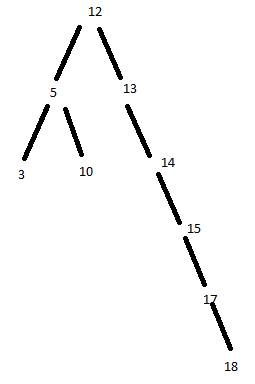
\includegraphics[scale=0.5]{arbre.png}
\paragraph*{Question 4(Ivan)}
\\

Voir arbre ci-dessus pour les clés insérées. On sous-entend ici que comme la valeur 15 s'y trouve déjà, on ne la rajoute pas une deuxième fois. Autrement, la valeur 15 serait l'enfant gauche du noeud contenant déjà cette valeur. 
\\

S'il s'agissait d'un arbre (2,4), l'arbre n'aurait que des enfants avec entre 2 et 4 noeuds (voir illustration ci dessous.)
\\
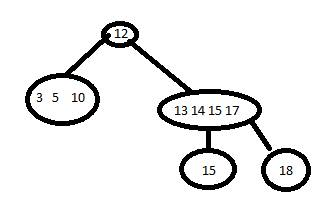
\includegraphics[scale=0.6]{arbre1.png}
\\
Si l'arbre était un B-arbre d'ordre 4 il aurait été pareil que l'arbre ci-dessous car les deux types contiennent des 4-Noeuds. Le Splay-tree aurait eu une apparence différente, la racine aurait été l'élément 10 avec comme enfant droit 12, et 12 aurait comme enfant droit le sous-arbre droit du premier graph.
\\

\newpage
\paragraph*{Question 5 (Wojciech GRYNCZEL)\\}
\textbf{L’ordre d’insertion des clés dans un AVL a t-il une influence sur la forme finale de l’arbre ?}
L’ordre d’insertion n’influence pas toujours la forme finale de l’arbre. Par exemple si on insère  les clés  (1) (2) (3) dans n’importe quel ordre, la forme finale sera toujours même: \\
\begin{center}
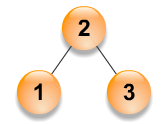
\includegraphics{tree1}
\end{center}

Mais si on insère plus de clés, la forme finale change.\\
\begin{center}
(2) (5) (6) (13) (15) (48) (1)\\
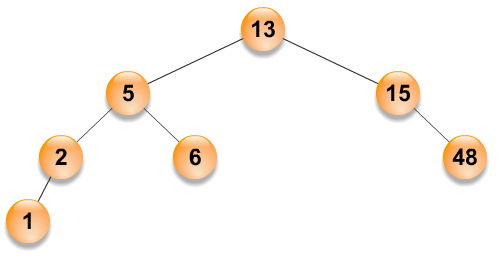
\includegraphics{tree2}\\
(1) (48) (15) (13) (6) (5) (2)\\
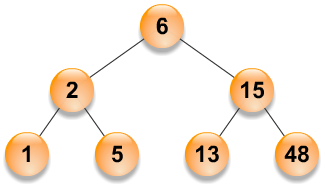
\includegraphics{tree3}
\end{center}
\newpage
\textbf{Dessinez un arbre AVL de hauteur 5 ayant un nombre minimal de nœuds :}\\
\begin{center}
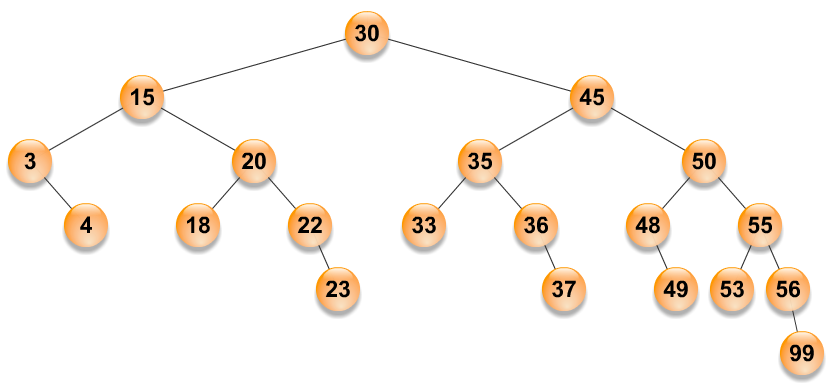
\includegraphics[scale=0.8]{tree4}
\end{center}
\textbf{Que peut-on dire de la relation entre hauteur h et nombre de noeuds n dans un arbre AVL ?}\\
La hauteur est toujours logarithmique en fonction de la taille de l’arbre.

{\footnotesize Soucres : \\
http://pauillac.inria.fr/~maranget/X/421/poly/arbre-bin.html\\
http://www.qmatica.com/DataStructures/Trees/AVL/AVLTree.html\\
http://pegasus.cc.ucf.edu/~fgonzale/eel4851/avltrees.PDF\\}

\paragraph*{Question 6 (Rodolphe Cambier)}


L'algorithme utilisé est le suivant:

On prend l'élément le plus petit de l'arbre U, et on insère celui-ci à la hauteur 2*(hauteur(U))-1 dans l'arbre T.

Faisant cela, on garde U comme sous-arbre à l'emplacement où l'on vient de rajouter l'élément. Mais on supprime l'élément de ce sous-arbre.

Il suffit ensuite de régler l'overflow éventuel et les deux arbres sont fusionnés.

\begin{figure}[H]
\centering
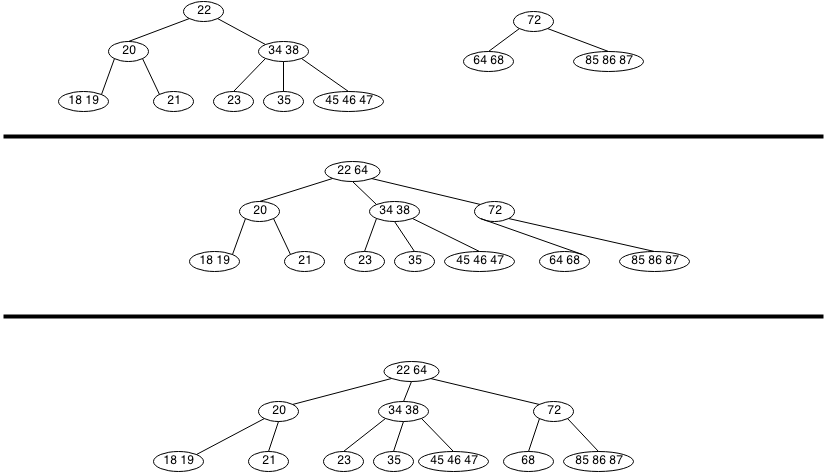
\includegraphics[scale=0.5]{algo.png}
\caption{On insère (64) à la hauteur 3 (2*2-1) dans l'arbre T, en lui laissant U comme sous-arbre. On supprime ensuite l'élément du sous-arbre U. Il n'y a ici pas d'overflow.}
\end{figure}

La complexité est la suivante (avec n = nbr de clés dans T et m = nbr de clés dans U):

On récupère le plus petit élément de U , O(log(m)) par définition de la fonction get().

On l'insère dans T, en gérant les overflows, O(log(n)) par définition de la fonction insert().

On supprime de T l'élément qui y est maintenant en double, O(log(n)) par définition de la fonction remove().

Donc on a O(log(n)) + 2*O(log(m)) = O(log(n)) + O(log(n) = O(log(n) + log(m)). 

\paragraph*{Question 7 (Bertaux Jérôme)}
\begin{enumerate}
\item Cas 1 :  Après l'ajout d'un élément, l'arbre est toujours équilibré : il n'est pas nécessaire d'effectuer une opération de rééquilibrage. (Voir figure 1a et 1b de l'annexe de l'énoncé)
\item Cas 2 : Après l'ajout d'un élément, l'arbre n'est plus un arbre AVL. Pour revenir à un arbre AVL, il faut rééquilibrer l'arbre par une simple rotation. (Voir figure 2a de l'annexe de l'énoncé)
\item Cas 3 : Après l'ajout d'un élément, l'arbre n'est plus un arbre AVL. Pour revenir à un arbre AVL, il faut rééquilibrer l'arbre par une double rotation.
\begin{center}
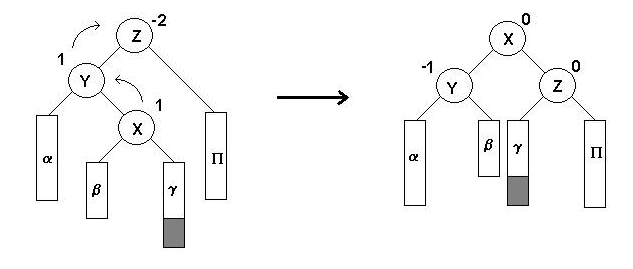
\includegraphics[scale=0.5]{double_rotation}
\end{center}
\end{enumerate}
{\footnotesize Soucres : \\
https://cours.etsmtl.ca/SEG/FHenri/inf145/Suppléments/arbres\%20AVL.htm\\}

\paragraph*{Question 8 (Baptiste Degryse)}
La propriété la moins évidente à vérifier est l'équilibre de l'arbre. Puisqu'il y a 1000 éléments, la profondeur de l'arbre doit être de maximum $log_2(1000) = 9.9 \simeq 10 $. Donc, pour la racine, il doit y avoir entre 512 et 488 clés dans chaque sous-arbre si toutes les clés sont utilisées. Sinon, il faut avoir un minimum de $2^{n-1}$ où n est la hauteur visible lors de la recherche.

2, 252, 401, 398, 330, 344, 397, 363 : Impossible, l'arbre n'est pas équilibré ( donc pas AVL ) car il y a maximum 1 enfant à gauche de la racine. (le chiffre 1)

924, 220, 911, 244, 898, 258, 362, 363 : $2^{7-1} = 64$. Il n'y a donc pas de problème pour celui-ci, mais il y a une grande densité de présence de clé pour les clés élevées.

925, 202, 911, 240, 912, 245, 363 : idem

2, 399, 387, 219, 266, 382, 381, 278, 363 : Impossible, l'arbre n'est pas équilibré ( donc pas AVL ) car il y a maximum 1 enfant à gauche de la racine. (le chiffre 1)

935, 278, 347, 621, 299, 392, 358, 363 : il faut 64 éléments dans l'autre sous arbre, ce qui implique que toutes les clés sauf une doivent être présentes au dessus de 934 pour que l'arbre soit valide.


\end{document}
